\documentclass[aspectratio=169]{beamer}

\usepackage[utf8]{inputenc}
\usepackage[TS1,T1]{fontenc}
\usepackage{amsmath}
\usepackage{biblatex}
\usepackage{graphicx}
\usepackage{ctex}

\usepackage{tikz}
\usetikzlibrary{decorations.pathreplacing}

\addbibresource{references.bib} % Specify the bibliography file

\title{\Large{\bfseries{不定方程相关理论及其应用}}}
\date{\scriptsize{\today}}
\author{\small{\fangsong{郑欢誉}}}

\usetheme[language=english]{LTU}

\begin{document}
	
	\begin{frame}
		\titlepage
	\end{frame}
    
   	\begin{frame}{开题报告目录}{\small{Contents of Thesis Proposal}}
       \liwicki[1]{研究背景和意义\small{Research Background \& Significance}}\\
       \liwicki[2]{文献调研\small{Literature Research}}\\
       \liwicki[3]{研究方案和进度安排\small{Research Scheme \& Scheduling}}\\
   	\end{frame}
	
	\begin{frame}{研究背景和意义}{Research Background \& Significance}
		$$
        x^n + y^n = z^n
        $$
        \begin{quote}
            \begin{enumerate}
                \item[1637] 费马:提出猜想
                \vspace{5pt}
                \item[1839] $n=3, 4, 5, 7$,无穷递降
                \vspace{5pt}
                \item[1847] \textbf{库默尔:唯一分解,理想};
                %\vspace{2pt}
                $n$ \underline{正规素数}(不整除$\mathbb{Q}(\zeta_n)$的类数)
                \vspace{5pt}
                \item[1994] 怀尔斯:模形式和椭圆曲线
            \end{enumerate}
        \end{quote}
	\end{frame}
	
	\begin{frame}{文献调研}{Literature Research}
    $$
    x^n+y^n=z^n \ \text{对任意的} \ n > 2 \ \text{无整数解} \ (x, y, z)
    $$
    \begin{flalign}
    \notag
    \overset{\text{分析}}{\implies} &\text{只需要考虑} \ \underline{n=p \ \text{为奇素数}} \ \wedge \ \underline{x,y,z \ \text{互素}}\text{的情况}\\
    \notag
    \overset{\text{在} \mathbb{Q}(\zeta_p) \text{中}}{\implies} &\underline{(x+y)(x+\zeta_p y)\cdots (x+\zeta_p^{p-1} y)=z^p} \Leftarrow \text{在} \mathbb{Z}[\zeta_p] \text{中分解}
    \end{flalign}
	\end{frame}
    
    \begin{frame}{文献调研}{Literature Research}
    \begin{center}
    \textbf{“在数域中唯一分解在什么程度上失效或保持?”}
    \end{center}
    \liwicki[1]{所讨论的分解是在什么子环上进行的?$\implies$ \underline{整数环}}\\
    \liwicki[2]{修复唯一分解 $\implies$ \underline{理想}}\\
    \liwicki[3]{度量唯一分解失效的程度?$\implies$ \underline{类数}}\\
    \liwicki[4]{简化素理想在分解中的行为 $\implies$ \underline{正规素数}}\\
    \liwicki[5]{整数环里可逆元组成的群的结构?$\implies$ \underline{单位定理}}
    %\begin{enumerate}
    %\item \textit{factorization with respect to what subring?} $\implies$ \underline{ring of integers}
    %\item recovering unique factorization $\implies$ \underline{ideal}
    %\item \textit{a way to measure by how much unique factorization fails?} $\implies$ \underline{class number}
    %\item simplifying how prime acts $\implies$ \underline{regular primes}
    %\item \textit{the structure of the group of units in the ring of integers?} $\implies$ \underline{unit theorem}
    %\end{enumerate}
    \end{frame}
    
    \begin{frame}{文献调研}{Literature Research}
    库默尔:将问题(正规素数情况)拆分为 \\
    \begin{center}
    $x,y,z$ \underline{均与 $p$ 互素} v.s. \underline{恰有一个被 $p$ 整除}
    \end{center}
    \begin{equation}
    \notag
    \begin{matrix}
        \prod_{i=0}^{p-1}\langle x+\zeta_p^iy\rangle = \langle z\rangle^p & \mid & \prod_{i=0}^{p-1}\langle x+\zeta_p^iy\rangle = I^{pm} \langle z_0\rangle^p
    \end{matrix}
    \end{equation}
    \end{frame}
    
    \begin{frame}{文献调研}{Literature Research}
    \textbf{FLT \& ABC 猜想}:\\
    \vspace{10pt}
    (ABC猜想):$\forall \epsilon > 0$, $\exists k_\epsilon$ s.t. 对任意满足 $a+b=c$ 的互素的 $a, b, c$,
    $$
    c \leq k_\epsilon \left(\prod_{p \ \text{素数}, \ p \mid abc} p\right)^{1+\epsilon}
    $$
    \begin{itemize}
    \item ABC $\implies$ FLT(Goldfeld, 1999)
    \item ABC猜想次指数界的改良(Hector, 2024)
    \end{itemize}
    \end{frame}
    
    \begin{frame}{文献调研}{Literature Research}
    \textbf{渐进费马大定理(Asymptotic Fermat's Last Theorem)}:\\
    \vspace{10pt}
    (渐进FLT): $K$ 为一个数域,存在一个仅依赖于 $K$ 的界 $B_K$,使得对任意的素数 $p > B_K$,下面的丢番图方程无非平凡解
    $$x^p + y^p + z^p = 0$$
    \begin{itemize}
    \item 通过 \underline{类域论}在无穷族数域上建立了渐进费马大定理(Freitas, 2020)
    \end{itemize}
    \end{frame}
    
    \begin{frame}[fragile]{文献调研}{Literature Research}
    \textbf{正规素数情况的形式化}(Riccardo, 2024):\\
    \begin{figure}
 		\centering
 		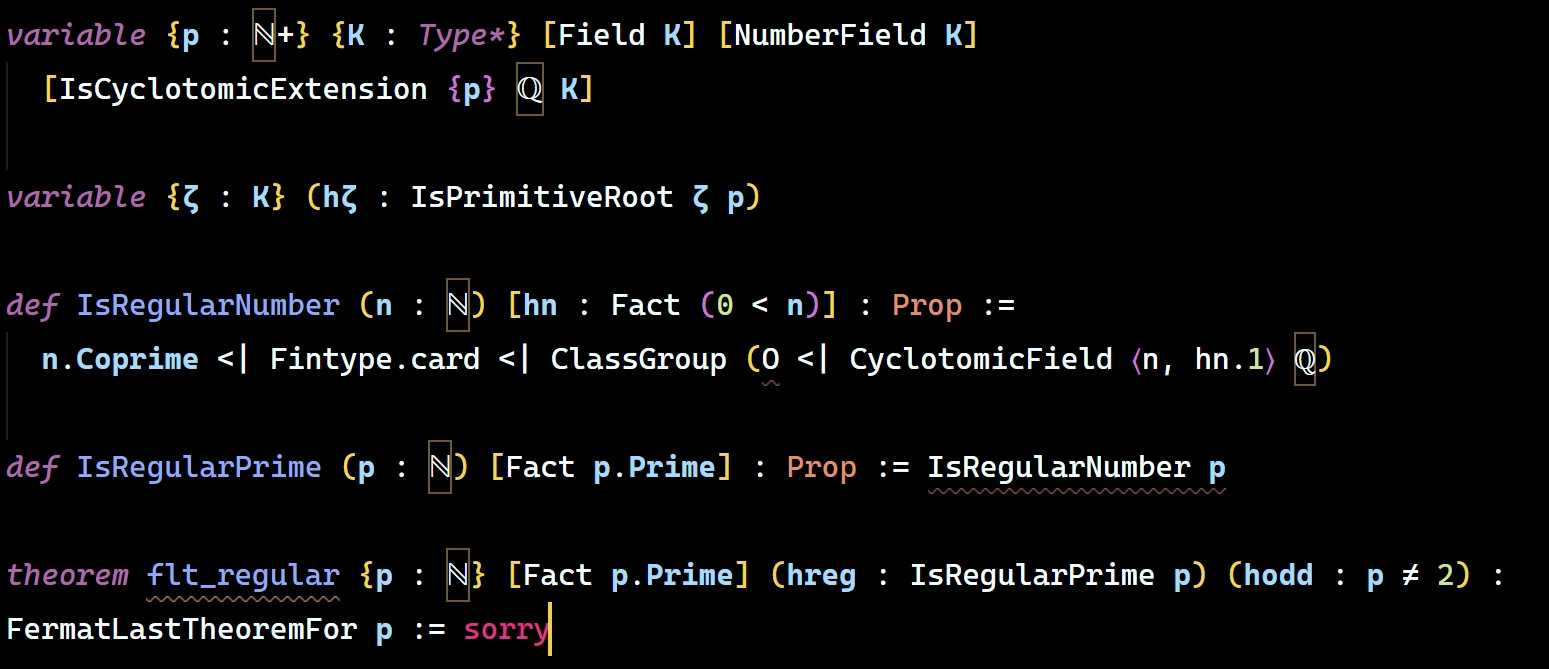
\includegraphics[width=0.8\linewidth]{screenshot.png}
	\end{figure}
    \end{frame}
	
	\begin{frame}{研究方案和进度安排}{Research Scheme \& Scheduling}
    \begin{quote}
            %\begin{small}
            \begin{itemize}
                \item[1-2月] 
                代数数论和交换代数(Ian\&Tall,Ash,Milne,Matsumura)\\
                \vspace{3pt}
                理解掌握库默尔关于正规素数情况的证明
                \vspace{10pt}
                \item[2-3月]
                通过Hector和Andrew的工作学习费马大定理与ABC猜想间的关联\\
                \vspace{3pt}
                利用类域论拓展性地了解渐进费马大定理
                \vspace{10pt}
                \item[3-4月] 形式化相关工作
            \end{itemize}
            %\end{small}
    \end{quote}
    \end{frame}
\end{document}